\documentclass[fleqn,10pt]{wlscirep}
\usepackage[utf8]{inputenc}
\usepackage[T1]{fontenc}
\title{Direction-Selective Resistance to Cerebrospinal-Fluid Flow As
the Mechanism of Syrinx Generation in Syringomyelia}

\author{Han Soo Chang, M.D.}
\affil{Department of Neurosurgery, Tokai University\\Isehara, Japan}

\keywords{syringomyelia, pathophysiology, simulation}

\begin{abstract}
    The pathophysiology of syringomyelia is not well understood. The main
    theoretical problem is how cerebrospinal fluid (CSF) enters from
    low-pressure subarachnoid space to high-pressure syrinx and stays
    there.
\end{abstract} \begin{document}

\flushbottom
\maketitle
% * <john.hammersley@gmail.com> 2015-02-09T12:07:31.197Z:
%
%  Click the title above to edit the author information and abstract
%
\thispagestyle{empty}

\noindent Please note: Abbreviations should be introduced at the first mention in the main text – no abbreviations lists. Suggested structure of main text (not enforced) is provided below.

\section*{Introduction}

The pathophysiology of syringomyelia is still poorly understood. A number
of hypotheses exist in the literature \cite{gardner1958mechanism,
williams1980pathogenesis, milhorat1999chiari, ball1972pathogenesis,
klekamp2002pathophysiology, duboulay1974mechanism, heiss1999elucidating,
milhorat1993anatomical, stoodley2000pathophysiology, terae1994increased,
chang2003hypothesis, chang2004theoretical, greitz2006unraveling}, but
they provide widely different explanations on the mechanisms of syrinx
generation.  Most researchers, nevertheless, seem to agree on the following
points. First, the syrinx fluid is identical to the CSF, and there should
be some communication between the syrinx and the subarachnoid space. This
point is supported by many studies \cite{ellertsson1969syringomyelia,
ellertsson1969myelocystographic, li1987conventional, heiss2019origin},
although a few different opinions exist \cite{greitz2006unraveling,
koyanagi1997surgical}. Second, some derangement of CSF flow in the spinal
subarachnoid space causes syrinx both in Chiari-I malformation
\cite{wolpert1994chiari, bhadelia1995cerebrospinal, heiss1999elucidating,
hofmann2000phasecontrast, quigley2004cerebrospinal} and subarachnoid
arachnopathy \cite{klekamp1997treatment, brodbelt2003altered,
heiss2012pathophysiology, chang2014dorsal}. The cerebellar tonsils hamper
the CSF flow in the former and adhesive arachnoiditis in the latter.

The problem, however, is where this communicating channel resides and what
mechanism generates the syrinx. On these points, there is no solid
experimental or clinical evidence, and the opinions of researchers deviate
widely. Gardner et al. \cite{gardner1958mechanism} thought that the central
canal intercommunicates the syrinx and the fourth ventricle, and arterial
pressure waves exerted on the central canal generate the syrinx. Williams
et al. also postulated the communication through the central canal, but for
the syrinx generation mechanism, he emphasized the craniospinal pressure
gradient produced by Valsalva maneuver et al
\cite{williams1980pathogenesis}.

On the other hand, Ball and Dayan \cite{ball1972pathogenesis} assumed that
CSF enters the syrinx through the perivascular space of arteries
penetrating the spinal cord. This idea has the following variations. Heiss
et al.  \cite{heiss1999elucidating} proposed that the piston-like movement
of the cerebellar tonsils in Chiari-I patients generates pressure waves in
the spinal subarachnoid space, which subsequently drive CSF into the syrinx
through the perivascular space. Stoodley et al. also considered the
perivascular space as the communicating channel, but he assumed the
arterial pulse pressure as the driving force of CSF
\cite{stoodley2000mechanisms} All these assumptions are not proven and
remain hypothetical. Although the perivascular-space theory seems to be
favored by recent researchers, there remains the possibility that a thin
communicating channel exists between the syrinx and the fourth ventricle
\cite{chang2021hypothesis}. 

In our opinion, the main theoretical problems reside in the following
points.
\begin{enumerate}
    \item No theory can explain the pathophysiological mechanism of
syringomyelia in a unified fashion.
    \item No theory can explain how CSF enters from the low-pressure subarachnoid space to the high-pressure syrinx cavity and remains inside.
\end{enumerate}

As to the first point, there are different syringomyelia types, such as
Chiari-I-malformation and spinal-arachnopathy-related
\cite{klekamp1997treatment}. The Chiari-I-malformation-related
syringomyelia is further divided into communicating and non-communicating
\cite{elliott2013syringomyelia}. For each of them, current theories assume
a distinct mechanism of syrinx generation. However, it may be more natural
to conjecture some common mechanism underlying these different types of
syringomyelia \cite{stoodley2000mechanisms}.  The second point is
theoretically essential but challenging to solve. Physical theories dictate
that the expanded syrinx cavity has higher pressure than the subarachnoid
space \cite{serwayr.a.2016fluids, heiss1999elucidating,
davis1989mechanisms, ellertsson1970distending}. Therefore, merely assuming
a communicating channel does not explain how CSF enters the syrinx and
remains inside against this pressure gradient. Even if we take a specific
time window where the subarachnoid pressure exceeds the syrinx pressure, it
does not explain how the CSF remains inside the syrinx after it.

The current article is part of our effort to solve the above theoretical
problems. In our previous paper \cite{chang2021hypothesis}, we hypothesized
that if there is a resistance to CSF flow in a particular direction
(rostral or caudal), it causes a one-way valve-like effect on a CSF channel
inside the spinal cord, leading to the accumulation of CSF and generation
of a syrinx. This hypothesis was attractive to us because it could explain
the pathophysiology of both Chiari-I-malformation-related syringomyelia and
arachnopathy-related syringomyelia. Namely, in
Chiari-I-malformation-related syringomyelia, the herniated cerebellar
tonsils may function as a direction-selective resistance. In
arachnopathy-related syringomyelia, some arachnoid adhesion may play the
same function \cite{chang2014dorsal}.  However, in that article, we just
drew a rough sketch of this process and left out a detailed explanation.
The current article will describe in detail how direction-selective
resistance in the subarachnoid space generates a one-way valve mechanism in
the CSF channel inside the spinal cord.

For this purpose, we used a mathematical model simulating the CSF movement
of the spine---a revised version of our previous model \cite{chang2003hypothesis,
chang2004theoretical}. This model describes the spinal CSF movement as an
electric current in a modeled circuit (a lumped parameter model with
multiple compartments \cite{shi2011review}), and it assumes the existence of a
patent central canal. We placed a direction-selective resistance in this
model at a certain point in the spinal subarachnoid space and observed how
it affects the CSF flow in the central canal.

\section*{Material and Method}

Some problem exists in the computer simulation of the motion of biological
fluids such as blood and CSF. Such bodily fluids move inside flexible
tubes. It, therefore, requires different analysis techniques from those
used in the engineering field, where the boundary of the conduit is
supposed to be solid. For this purpose, researchers widely used lumped
parameter models \cite{shi2011review, @kokalari2013review}. This model
considers the fluid flow inside a flexible tube in analogy to the flow of
electricity in an electric circuit. The accumulation of electricity in a
capacitor represents the expansion of a flexible tube and the accompanying
pressure elevation. An electrical resistor represents the frictional
resistance to flow. This model has a wide variety. For example, it may
model the whole cardiovascular system as one electric circuit, or it may
model it as a synthesis of multiple compartments of electric circuits
[@shi2011review; @kokalari2013review]. Our current model is the type of a
lumped parameter model with multiple compartments.  In this study, we did
not intend to make a quantitatively precise model of the spinal CSF flow
but to make a basic model that reveals the phenomenon underlying the
generation of syringomyelia. For this purpose, we adopted a revised version
of our previous lumped parameter model with multiple compartments.

Previously, we developed a mathematical model that simulated the CSF flow
in the spine \cite{chang2003hypothesis, chang2004theoretical}. This model (a
multiple-compartment version of a 1-dimensional lumped parameter model)
could describe the CSF movement in the whole spine (Figure \ref{fig:model}).

\begin{figure}[ht]
    \centering
    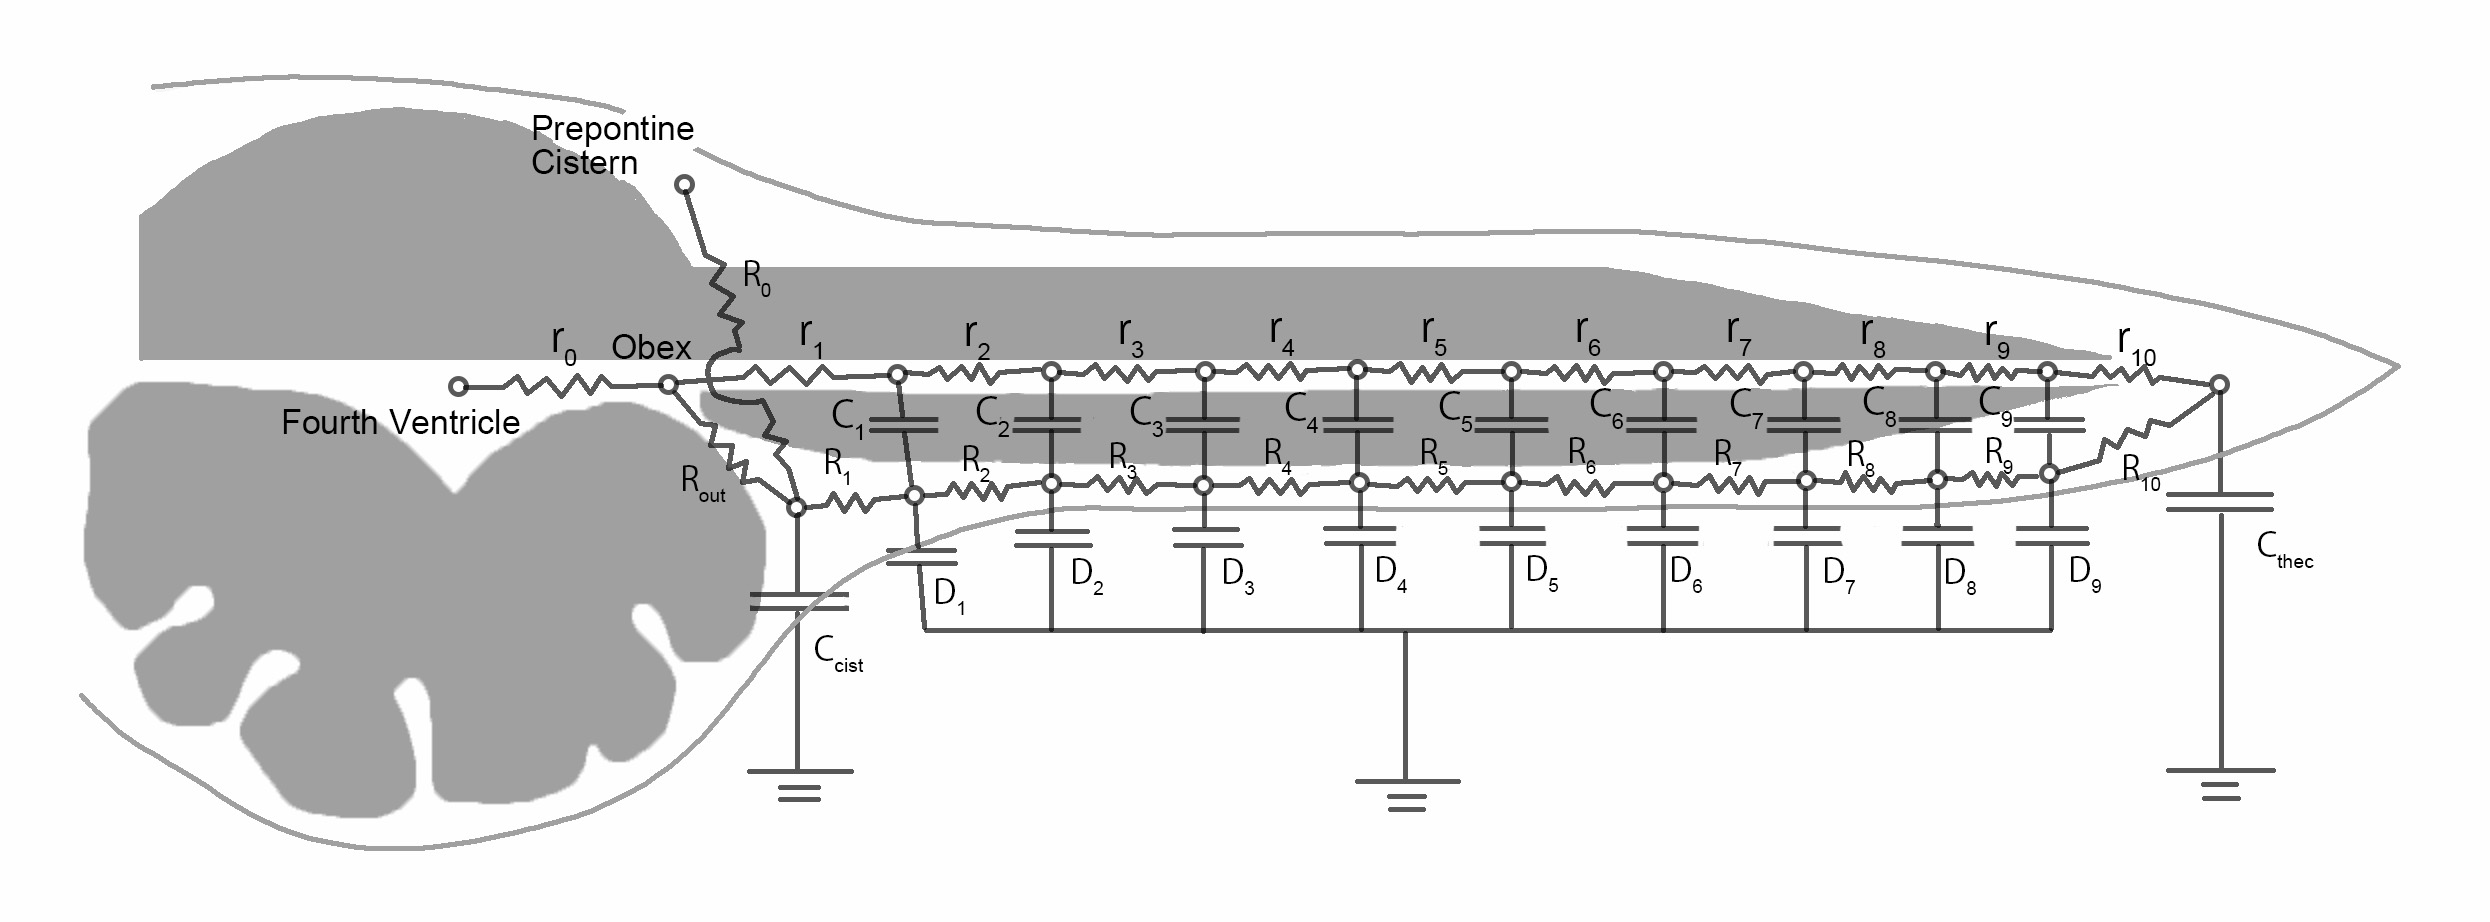
\includegraphics[width=\textwidth]{ps_circuit_schema.jpg}
    \caption{Schema of the electric circuit model of the CSF dynamics in the
    spine.}
    \label{fig:model}
\end{figure}

A set of differential equations can describe the behavior of this model.
Using computer software, we can numerically calculate its behavior to a
cranial pressure wave (defined as a boundary condition on the cranial
points).  This time, we improved the previous model as follows.

\begin{itemize}
    \item We increased the number of compartments from 10 to 100, thereby making the model more precise.
    \item We estimated the values of the parameters (the capacitance and resistance of each component) of the model as follows so that the model will become more realistic.
        \begin{itemize}
            \item First, we set the length of the modeled spinal cord to be 1 meter.
            \item The resistance of the subarachnoid space ($R$) was
                estimated using the following equations of Poisseuille
                \cite{brook1999numerical, sherwin2003computational, huilgol2020fast}. 
             $$\Delta P=\frac{8\pi \mu{}LQ}{A^{2}}=RQ$$
                \begin{itemize}
                    \item $\Delta P$: Pressure difference between the adjacent compartments
                    \item Q: flow speed per unit surface
                    \item $\mu$: viscosity coefficient. In this case, it was set to the value of water (0.0007).
                    \item L: distance between the adjacent compartments. It was set to 1 cm.
                    \item A: cross sectional area of the subarachnoid
                        space. It was set to the value of a concentric
                        annulus \cite{huilgol2020fast} with the outer diameter of 1cm and the inner diameter of 0.7 cm ($1.6\times{}10^{-4} (m^2)$) 
                \end{itemize}
            \item Thus, $R$ was calculated to be $6872\hspace{0.2cm}(Pa\cdot{}sec/m^3)$
            \item The resistance of the central canal ($r$) was estimated
                using the same equation with $A$ set to
                $\pi{}(10^{-4})^2\hspace{0.1cm}(m^2)$, i.e. the cross
                sectional area of a tube with a diameter of 100 $\mu{}m$.
                Thus, $r$ was calculated to be $1.78\times10^{11}\hspace{0.2cm}(Pa\cdot{}sec/m^3)$
        \end{itemize}
    \item We determined the capacitance ($C_{sub}$)corresponding to the dural elasticity so that the pressure-wave velocity determined by the time constant ($RC$) will roughly correspond to the pressure-wave velocity of the downward CSF wave observed in phase-contrast MRI of normal individuals. Thus, we set $C_{sub}=0.1\hspace{0.2cm}(m^3/Pa\cdot{}sec)$.
\end{itemize}

Figure 1 shows the scheme of the constructed electric circuit model. This
model represents the CSF movement in the spine as electric flow through
multiple compartments of capacitances connected with resistors. Table 1
shows the values of the resistors and capacitors of the system.  A set of
differential equations can describe the behavior of this electric circuit,
and we can solve it numerically by setting the voltage at the cranial nodes
as the boundary condition (Figure \ref{fig:circuit}). In the previous articles
\cite{chang2003hypothesis, chang2004theoretical}, we only analyzed the
transient behavior of the model to a sudden pressure increase on the
cranial side of the subarachnoid space. This analysis helped simulate the
situation of coughing or Valsalva maneuvers. In this article, however, we
analyzed the steady-state response of the model to an oscillating cranial
pressure wave simulating the normal cardiac pulsation of the CSF.

\begin{figure}[ht]
    \centering
    \includegraphics[width=\textwidth]{electric_circuit_new.jpg}
    \caption{Electric circuit diagram representing the CSF dynamics of the spine}
    \label{fig:circuit}
\end{figure}

We numerically solved the differential equations using computer software
(Mathematica version 12, Wolfram Research, Champaign, IL, U.S.A.). We set
the boundary conditions as follows. (1) The voltage at the two cranial
nodes was set to a sine wave oscillating around 100 mmHg with an amplitude
of 20 mmHg at one cycle per second. (2) The initial dural pressure was set
at 100 mmHg in all segments. We set the step of the numerical solution to
1/5000 second and calculated the solution from zero to 20 seconds. We
displayed the obtained solution as a movie in mp4 format.

We analyzed the original normal system and two of its modifications.

\section*{Results}

We present the system's responses as videos. Each video displays either all
or some of the following four values simultaneously: namely, the dural
tension (voltage in D capacitors in Figure 2), the canal tension (voltages
in C capacitors), the subarachnoid CSF flow (flows in R resistors), and the
canal flow (flows in r resistors). We plotted the node position on the
x-axis and the values at that node on the y-axis. The pressure values are
shown in $cmH_2O$, the flows in $ml/sec$. To plot different ranges of
values in a single plot, we multiplied the following values with certain
coefficients: namely, the canal tension with 50, the subarachnoid flow with
0.005, and the canal flow with $1.5\times10^{5}$. We plotted the
rightward flow in the positive and the leftward flow in the negative
direction.  Video 1 shows the original system's response to the sine wave
input on the cranial side. In this condition, CSF makes a smooth to-and-fro
movement in the subarachnoid space with the corresponding pressure wave
along the dura and the central canal. This response corresponds to the CSF
dynamics in a normal individual.

In Video 2, we increased the subarachnoid resistance $R_{25}$ by 20
times, thereby simulating a simple block of the subarachnoid flow in both
directions. In this condition, the dural tension showed a pressure drop at
node 25, corresponding to the increased resistance both in caudal and
rostral flow phases. This pressure drop caused an increase in canal flow in
a direction identical to the subarachnoid CSF flow. This increased canal
flow caused a transient increase in canal pressure distal to the block and
a decrease proximal to the block. However, these pressure changes
alternated according to the flow phase and did not produce a sustained
condition.

In Video 3, we replaced the subarachnoid resistor $R_{25}$
with a one-way valve that selectively resisted flow in the caudal direction
by 50 times. This time, the dural tension curve showed a pressure drop
across node 25, appearing only during the caudal-flow phase. Canal flow
showed alternating increase in caudal and rostral directions according to
the flow phase, which was similar to that in the simple block above.
However, there was a significant difference. Sustained high pressure
appeared in the central canal distal to the valve, and some sustained low
pressure in the segment proximal to the valve. The canal flow near node 25
markedly increased caudally in the caudal-flow phase and rostrally in the
rostral-flow phase. We took out the canal flow and showed it in Video 4.
Observing this video, we can see that the cumulative total of the caudal
flow is larger than that of the rostral flow, and it means that the CSF is
virtually pumped caudally at node 25. 


\section*{Discussion}

In this article, we theoretically analyzed the CSF movement in the spinal
cord using a lumped parameter model with multiple components. It simulated
a system with an elastic tube (dura) containing an elastic cylindrical
material (spinal cord) that itself contained a fluid channel (the central
canal). When we placed a direction-selective resistor in the subarachnoid
channel and evoked a to-and-fro pressure wave on this system, it produced a
sustained pressure elevation in the segment distal to the
direction-selective resistor. This phenomenon may explain the pathogenesis
of syringomyelia both in Chiari I malformation and syringomyelia associated
with arachnopathy.

Subarachnoid pressure affects the pressure inside the central canal. As
seen in Figure 2, the absolute pressure inside the central canal is the sum
of the subarachnoid and canal pressure (voltages of $C_k$ and $D_k$ in
electrical terms). Suppose a one-way valve selectively resists caudal flow
in the subarachnoid space at point A, and CSF makes a to-and-fro movement
across it. The caudal-flow phase creates a pressure drop across point A,
making the subarachnoid pressure in the distal segment smaller, and it
reduces the absolute canal pressure in the distal segment. Thus, the
pressure gradient in the central canal across point A increases, which
increases the distal CSF flow in the canal at that point.

On the contrary, the rostral flow does not create a pressure drop. Although
some of the CSF pumped caudally will flow back rostrally, its amount will
be smaller. The net result will be that some CSF is pumped caudally in one
cycle of the to-and-fro movement. Thus, CSF gradually accumulates in the
distal segment of the resistance. We hypothesize that this is the mechanism
underlying the syrinx generation.

This hypothesis solves the theoretical problems pointed out in the
Introduction. A one-way valve in subarachnoid space creates an asymmetry of
the pressure gradient between the caudal and rostral flow phases in the
central canal. This asymmetric alternation of pressure gradient effectively
pumps CSF caudally, creating sustained pressure elevation in the caudal
segment. In other words, the energy of the to-and-fro CSF movement is
translated via the one-way valve into the creation and sustenance of
syringomyelia.

Direction-selective resistance to CSF flow is not an imaginative assumption
but actually exists in patients. In Chiari-I malformation, the herniated
tonsils move like a ball-valve, displaced caudally during the caudal flow
and rostrally during the rostral flow. Higher velocity observed in the
phase-contrast MRI studies suggests that it selectively impedes the caudal
CSF flow more than the cranial flow. This direction-selective resistance
was demonstrated by Williams in direct measurements in Chiari-I patients
and became the basis of his theory \cite{williams1981simultaneous}.

Also, there is a possibility that some types of arachnoid pathology
function as one-way valves. In 2014, we reported a case of thoracic
arachnoid web associated with syringomyelia, in which phase-contrast MRI
detected one-way-valve-like behavior of the arachnoid web
\cite{chang2014dorsal}. We found an obliquely oriented arachnoid web that
reminded us of a one-way valve in surgery. Thus, our hypothesis may also
solve the second theoretical problem that we pointed out in the
Introduction. Namely, we may consider the presence of a one-way valve in
spinal subarachnoid space as a common mechanism underlying both
Chiari-I-related and arachnopathy-related syringomyelia.  Our theory
assumes that the arterial-pulse generated to-and-fro CSF movement provides
the energy for syrinx generation. It is compatible with Stoodley et al.'s
experimental result that syrinx maintenance is dependent on arterial
pulsation \cite{stoodley2000mechanisms}. In this study, the authors showed that

\begin{center}
\includegraphics[width=\textwidth]{pumping_mechanism_close.jpg}
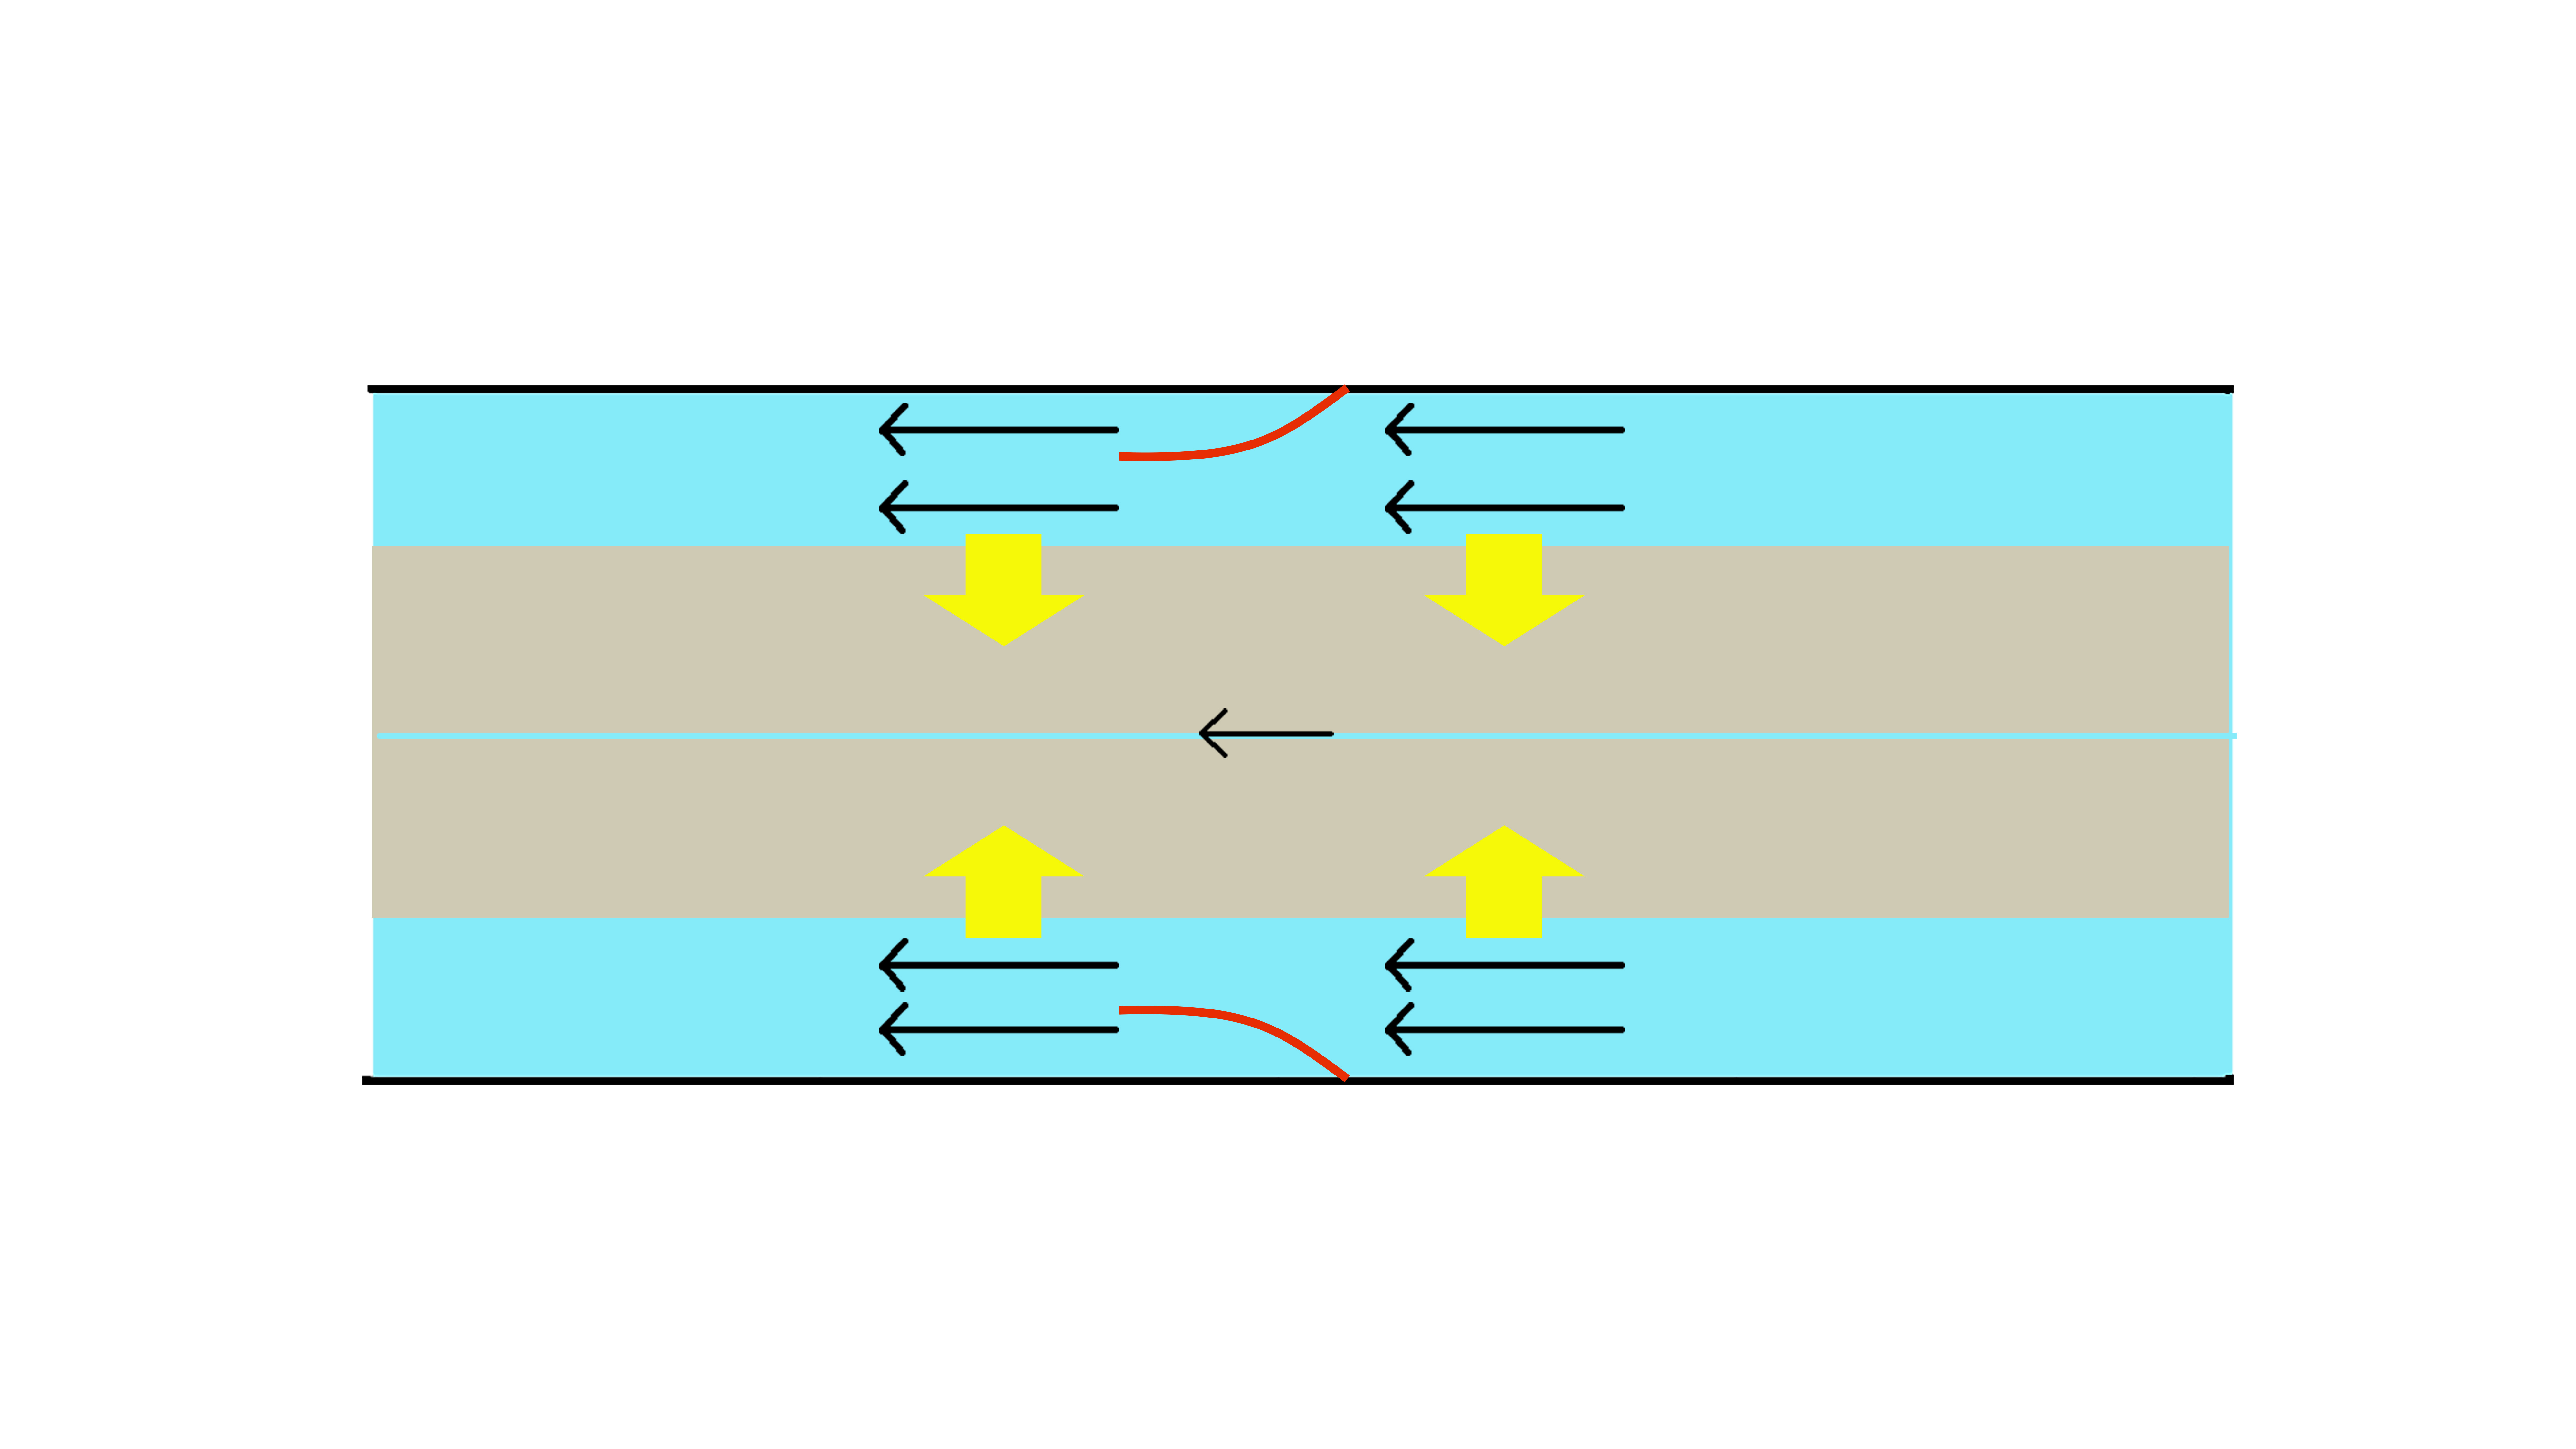
\includegraphics[width=\textwidth]{pumping_mechanism_open.jpg}
\end{center}

\bibliography{my_library}


\end{document}
